\cotefile{28}
\scanpage{2}
\uline{Demazure} 5.1.1970 \quad $\underline{\mathrm{Aut}}^{\circ}$

\uline{Introduction}
\diagram{\(\begin{array}{ll|l}
P_1\times P_1 && \mathrm{PGl}_2\times\mathrm{PGl}_2\\
P_2 && \mathrm{PGl}_{3}\deleted{\unsure{(3)|(G_3)}}\\
F_n & n\geq\deleted{\unsure{0|2}}1\quad(F_0=P_1\times P_1)
  & \bigl(\unsure{\mathrm{Gl}(2)|\mathrm{Gl}_2|\mathrm{GL}(2)}\mathbin{\cdot}\Gamma(\unsure{\mathcal O(n)|O(n)})\bigr)/\mu_n\\
 & (F_1=P_2\ \text{éclaté}) &
\end{array}\)}

\uline{Th.} (Enriques) : tout ss-gpe de $\mathrm{Cr}_2$, algébrique lisse connexe, est $\subset$ un des précédents à conjugaison près\ldots.

\uline{Cor.}
\[
\left\{\begin{aligned}
&\text{\deleted{\unsure{gpe}}\inserted{partie}}\ \text{réductive \uline{de type} }A_n\\
&\text{ils sont \uline{définis sur} }Z\\
&\text{sont des groupes d'autom. d'espaces très simples, \uline{proj. et lisses}}\\
&\text{(opérant avec orbites ouvertes)}\\
&\text{tous de rang }2
\end{aligned}\right.
\]

On va généraliser à la dim $n$, sauf difficulté liée aux tores maximaux ; OK si on prend les ss-groupes de \uline{rang maximum}

\uline{Sorites} \quad (Cas $X$ lisse séparé \inserted{\unsure{t.f.p.|t.f.}} sur $S$)

Pseudo-morphismes, pseudo-isomorphismes (rel/$S$)

Pseudo-automorphismes \(\mathrm{Psaut}_S(X),\quad\underline{\mathrm{Psaut}}_S(X)\)
\[
\begin{aligned}
&\underline{\mathrm{Psaut}}_k(K),\qquad
\underset{\sim}{\mathrm{Cr}}_{n,k}=\underline{\mathrm{Psaut}}_k(k[\unsure{t_1,-,t_n|t_1,\ldots,t_n}])\\
&\underline{\mathrm{Psaut}}_k(K)(k)\simeq\mathrm{Aut}_k(K)^{\circ}\\
&\mathrm{Lie}(\underline{\mathrm{Psaut}}_k(K))\simeq\mathrm{Der}_k(K)^{\circ}
\end{aligned}
\]

\uline{Proposition} Section unité de $\underline{\mathrm{Psaut}}_S(X)$ imm. fermée dans chacun des 2 cas

a) $S$ artinien

b) fibres \inserted{\unsure{géomt|géom.}} irréductibles

% archive sheet number: 1
\scanpage{3}
\uline{Cor} \(\underset{\substack{\text{schéma en}\\\text{groupes}}}{G}\xrightarrow{\text{hom de gp}}\underline{\mathrm{Psaut}}_S(X)\) Alors le noyau est un ss-schéma en groupes fermé

\deleted{\uline{Prop. 2} $X$ courbe irréductible propre\inserted{ sur $k$ corps}, $S$ loc. noeth. normal}

\deleted{$\underline{\mathrm{Psaut}}_S(X)$}

\uline{Lemme} \(\underset{\substack{\text{sch. en}\\\text{groupes}}}{G}\longrightarrow\underline{\mathrm{Psaut}}_k(X)\), $X$ courbe lisse propre sur $k$, il se factorise par $\deleted{\mathrm{Psaut}}\ \underline{\mathrm{Aut}}_k(X)$.

On \uline{fixe} corps $k$, et $X$ (lisse séparé t.f. /$k$)

Que signifie \(\underset{\substack{\text{schéma en}\\\text{groupes lisse}\\\text{de t.f.}}}{G}\xrightarrow{u}\underset{\sim}{\mathrm{Psaut}}_k(X)\) ?

\(G\times X\xrightarrow{\text{pseudo }\varphi} X\) ouvert de définition $U$ (ne contient pas en général $e\times X$)

(PO 1) \(\mathrm{pr}_1\circ\varphi\) dominant

(PO 2) associativité

\diagram{\begin{tikzcd}[ampersand replacement=\&]
G\times G\times X \arrow[r,dash,"m_G\times X"] \arrow[d,dashed,"G\times\varphi"] \& G\times X \arrow[d,dashed,"\varphi"]\\
G\times X \arrow[r,dashed,"\varphi"] \& X
\end{tikzcd}}

\[
\begin{aligned}
&\mathrel{\rotatebox{-35}{$\Updownarrow$}}\\[-2pt]
&\left[\begin{array}{ll}
g,h\in G(S) & h.x\ \text{défini}\\
x\in G(S) & g(h.x)\ \text{défini}
\end{array}\right.
\mathrel{\vert\!\Longrightarrow}(gh).x\ \text{défini et égal \unsure{à|:} }g.(hx)
\end{aligned}
\]

$\exists N\subset G$ ($=\operatorname{Ker}u$) tel que $u$ soit \deleted{\unsure{nul}}\inserted{trivial} sur $N$ et on \unsure{trouve|tire} $G/N\hookrightarrow\underset{\sim}{\mathrm{Psaut}}_k(X)$.

% archive sheet number: 2
\scanpage{4}
\diagram{\begin{tikzcd}[ampersand replacement=\&,row sep=1.2em]
G\times X \arrow[r,dashed] \& X\times X\\[-3pt]
\rotatebox{-90}{$\supset$} \& {}\\[-3pt]
U \& {}\\[-3pt]
\rotatebox{-90}{$\supset$} \& {}\\[-3pt]
F \arrow[r] \& X \arrow[uuuu]
\end{tikzcd}}

Opération \uuline{régulière} si $F\mathbin{-} X$ fid. \unsure{plats|plate|plat}

\uline{Prop} Si l'opération est régulière, $F_X$ est un sous-schéma en groupes de $G_X$.

\uline{Cor} $N$ est le plus \unsure{gd|grand} sous-schéma en groupes constant de $F_X$.

Pseudo-opération \inserted{(pseudo)}\uline{transitive} si $G\times X\mathbin{-}X\times X$ \uline{dominant}

(dans le cas d'une vraie opération, cel signifie qu'il y a une \inserted{(unique)} orbite dense)

\uline{Proposition} Si $G$ est pseudo-transitive sur $X$, $X$ est pseudo-isomorphe à un espace homogène.

\uline{Sous-tores de} $\underset{\sim}{\mathrm{Cr}}_{n,k}$ \uuline{Prop} Soit $T$ tore (\unsure{supp|qq} déployé) qui pseudo-opère de façon \deleted{\unsure{régulière}} \deleted{\unsure{effective}} \inserted{fidèle} régulière, \inserted{($X$ irréductible)} Alors $F=e\times X$

\deleted{\unsure{($X$ un|($X$ réd.}}

\uline{Cor} 1 $\dim T\leq\dim X$, égalité $\Longleftrightarrow$ pseudotransitivité

\uline{Cor.} 2 Supposons $\dim T=\dim X$, \inserted{$T$ déployé} Alors $X$ \deleted{$\unsure{\simeq|\approx}$}\inserted{torseur sous}\inserted{$G$-pseudoisomorphisme} $T$

\uline{Cor} 3 $X$ irréductible \inserted{dim $n$}, alors conditions équivalentes

a) $X$ rationnel

b) $\underline{\mathrm{Psaut}}(X)\simeq\underline{\mathrm{Cr}}_{n,k}$

c) $\underline{\mathrm{Psaut}}(x)\supset\unsure{\mathbb G_m^n|G_m^n}$

% archive sheet number: 3
\scanpage{5}
\uline{Cor. 4} Les tores déployés \inserted{de dim $n$} de $\underline{\mathrm{Cr}}_{n,k}$ sont conjugués.

\uline{Cor.} 5 Ils sont maximaux, ils sont leurs propres \unsure{centralisateur|centralisateurs}, et le normalisateur est un groupe \deleted{\unsure{lisse|tore}} lisse, et $N/T\simeq\underline{\mathrm{Aut}}_{\mathrm{gr}}(T)$.

\uline{Cor.} 6 $T$ est un tore maximal de $\underline{\mathrm{Cr}}_{n,k}$

\uline{Proposition} $T$ déployé, $X$ irréductible, pseudo-opération fidèle. Alors $X\overset{\text{\unsure{pseudo}}}{\sim}T\times Y$, où $Y$ est un schéma irréductible (unique à pseudo-isom près).

\uline{Cor} 1 Soit $0\leq d\leq n$. Conditions équivalentes

a) \unsure{Tous|Tout|Im} $G_m^d\subset\underline{\mathrm{Cr}}_{n,k}$ est contenu dans un $G_m^n$

b) Toute extension $K/k$ de degr. tr. $d$, \unsure{dt|et} $K[t_1,-,t_{n-d}]$ pure, est pure (``Lüroth'').

[\uline{NB} \quad OK si $d=0$, $d=1$, $d=2$ $\left|\begin{array}{l}\text{car. nulle}\\ k\ \text{alg. clos}\end{array}\right.$ (Castelnuovo).

\hspace*{4em}$d=n$

Marche si $n\leq 3$ \quad ]

\uline{Pb} Classifier les $G$ alg. lisses $\subset\underset{\sim}{\mathrm{Cr}}_{n,k}$ qui contiennent un tore déployé de dim $n$.

\uline{\unsure{Th. des actions|Th. de dém.|Th. de structure}}

On va fixer $T$, et chercher
\[
T\subset G\subset\underset{\sim}{\mathrm{Psaut}}(T)
\]
L'opération de $G$ sera transitive. On veut espaces homogènes $X$ sous $G$, de dim $n$, de telle façon que $T$ opère fidèlement avec une orbite ouverte

% archive sheet number: 4
\scanpage{6}
Utilisant \unsure{th. gr|th. quo}, on aura

\diagram{\begin{tikzcd}[ampersand replacement=\&,row sep=.4em]
T\subset G \arrow[d,phantom,"\rotatebox{-90}{$\supset$}" description] \&[-1em]
{\left\{\begin{aligned}
&T\times H\mathrel{\unsure{-|\longrightarrow}}G\quad\text{imm. ouverte}\\
&\deleted{\unsure{T\cap H=e}}\quad\bigcap\ \text{conjugués de }H=e
\end{aligned}\right.}\\
\hphantom{T\subset{}}H \&
\end{tikzcd}}

On aura pseudomorphisme $\mathrm{pr}_1$
\diagram{\begin{tikzcd}[ampersand replacement=\&] G\arrow[r,dashed,"f"] \& T \end{tikzcd}}
\[
\begin{aligned}
&[\,\text{pseudo-opération est}\qquad (g,t)\mapsto f(gt)\,]\\
&\hspace{13em}\rotatebox{90}{$=$}\\[-2pt]
&\hspace{12em}t f(t^{-1}gt)
\end{aligned}
\]

\uline{Axiomes sur $f$}
\[
\left\{\begin{aligned}
1)\quad &f(gg')=f(gf(g'))\quad \text{(si }f(g')\text{ est défini, les 2 \unsure{mbs|sens} le}\\
&\hspace{16em}\text{sont simultanément)}\\
2)\quad &f\ \text{défini en tt pt de }T,\ \text{et y induit l'identité}\\
3)\quad &\text{Si }g,g'\in G(S),\ \text{et }f(gt)\equiv f(g't)\ \text{pour tt }t\ \ldots-,\\
&\text{alors }g=g'.
\end{aligned}\right.
\]

\[
\Longrightarrow \qquad f(tg)=tf(g)
\]

\figure{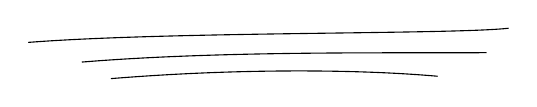
\begin{tikzpicture}[x=1cm,y=1cm]
\draw (0,0) .. controls (1.8,.14) and (5.4,.10) .. (6.1,.18);
\draw (.68,-.25) .. controls (2.5,-.10) and (4.8,-.14) .. (5.82,-.13);
\draw (1.05,-.46) .. controls (2.65,-.33) and (4.18,-.34) .. (5.2,-.43);
\end{tikzpicture}}
% archive sheet number: 5
\scanpage{7}
\uline{Demazure 12.2.\unsure{70|76}}

\diagram{\begin{tikzcd}[ampersand replacement=\&,row sep=.65em,column sep=.6em]
T \& \subset \& G \arrow[ll,bend right=26,dashed,"f"']\\
{} \& {\subset G'} \& \rotatebox{43}{$\subset$}
\end{tikzcd}}
possibilité de restreindre à un $G'$

\uline{Ex} \quad $G'=\mathrm{Centr}(\deleted{\unsure{T}}Q)$ \qquad $Q$ sous-tore de $T$

$\deleted{\unsure{S|R|\mathrm{N.B.}}}Q$ devient central.

Si $Z\subset T$ central dans $G$, alors on peut passer au quotient, les conditions 1) 2) 3) restent vérifiées (il faut un peu d'attention pour 3°)

\uline{Cas particulier} \quad $\dim G-\dim T=1$. $G$ n'est pas commutatif (car $T$ \uline{n'est pas} central si $T\neq G$)

On aura $G=T.\underset{\substack{\rotatebox{90}{$\simeq$}\\G_a}}{G_u}$ \quad produit $1/2$ direct donné par caractère non trivial

\uline{Proposition}
\diagram{\(\displaystyle\exists!\left\{\,\begin{tikzcd}[ampersand replacement=\&,row sep=.7em]
x_\alpha\colon G_a\arrow[r,"\sim"] \& U{,}\quad\text{et}\\
\rho_\alpha\colon G_m\arrow[r] \& T\arrow[l,bend left=26,"\alpha"]
\end{tikzcd}\right.\)}
t.q.
\[
\left\{\begin{aligned}
&t x_\alpha(\lambda)t^{-1}=x_\alpha(\alpha(t)\lambda)\\
&f(x_\alpha(\lambda))=\rho_\alpha(1+\lambda)\qquad
  (f\ \text{défini en }x_\alpha(\lambda)\ \text{ssi }1+\lambda\ \text{inversible})
\end{aligned}\right.
\]

\uline{De plus}, on aura
\[
\left\{\begin{aligned}
&\langle\rho_\alpha,\alpha\rangle=1\\
&H=x_\alpha(1)\deleted{\unsure{H}}T x_\alpha(-1)\qquad (?)
\end{aligned}\right.
\]

Inversement, si on se donne $\alpha,\rho_\alpha$ tels que $\langle\alpha,\rho_\alpha\rangle=1$, on reconstitue \ldots.

\uline{Cas général}

\diagram{\begin{tikzcd}[ampersand replacement=\&]
T \& \subset \& G \arrow[ll,bend left=30,dashed,"f"]
\end{tikzcd}}
\[
\begin{aligned}
&\mathfrak g=\underset{\substack{\rotatebox{90}{$=$}\\\underline{\mathrm{Lie}}\,T}}{\mathfrak g^{0}_{\deleted{\unsure{0}}}}
 +\sum_{\alpha\in R}\mathfrak g^\alpha
 \qquad R\subset\mathrm{Hom}(T,G_m)\\
&\hspace{8em}(T=\mathrm{Cent}_{\unsure{\mathrm{Cre}|\mathrm{Cr}|G}}\,T)\\
&\dim\mathfrak g^\alpha=1
\end{aligned}
\]

% archive sheet number: 6
\scanpage{8}
Soit $\chi:T\mathbin{-}G_m$
\[
\begin{aligned}
&T_\chi=(\operatorname{Ker}\chi)^\circ\subset T\\
&Z_\chi=\mathrm{Cent}(T_\chi)\\
&Z_\chi/T_\chi\quad\text{a comme tore maximal }T/T_\chi\\
&\hspace{7em}\text{de dim }1
\end{aligned}
\]

\diagram{\begin{tikzcd}[ampersand replacement=\&]
{} \& \unsure{\mathrm{Psaut}|\mathrm{Birat}|\mathrm{Baut}}(T/T_\chi)\\
Z_\chi/T_\chi\arrow[ur,dashed]\arrow[r,hook] \& {\mathrm{Aut}(\underline{\mathbb P}^{1})=\mathrm{GPL}(2)}\arrow[u,hook]
\end{tikzcd}}
\inserted{\unsure{car|cas} $P^1$ de dim 1}

4 possibilités pour ss-gpe de $\unsure{\mathrm{GBL}(2)|\mathrm{GPL}(2)|\mathrm{PGL}(2)}$ \unsure{contt} tore maximal
\diagram{\(\left\{\begin{array}{ll}
\text{tore maximal de }\mathrm{GPL}(2) &: Z_\chi=T\\
\text{son normalisateur} &: Z_\chi/T\ \text{de rang }2\\
\text{Borel} &\dim Z_\chi/T=1\\
\text{tout} &Z_\chi\ \text{réductif de rg}\\
&\boxed{1/2\ \text{simple }\underline{1}}
\end{array}\right.\)}

\uline{Conclusion} Supposons $\chi\in R$, les deux premiers \unsure{son|sont} exclus.

\textcircled{1} On trouve
\[
\begin{aligned}
&\left\{\begin{aligned}
 &\dim\mathfrak g_\alpha=1\\
 &\exists !\ x_\alpha:G_a\longrightarrow Z_\alpha\subset G,\qquad
 x_\alpha(G_a)=U_\alpha,\ \mathrm{Lie}(U_\alpha)=\mathfrak g_\alpha\\
 &\hspace{12em}t x_\alpha(\lambda)t^{-1}=x_\alpha(\alpha(t)\lambda)
\end{aligned}\right.\\
&\hspace{3em}\rho_\alpha:G_m\mathbin{-}T\qquad f(x_\alpha(\lambda))=\rho_\alpha(1+\lambda),\quad
 \langle\rho_\alpha,\alpha\rangle=1
\end{aligned}
\]

\[
\underline{\mathrm{Lie}}\, Z_\chi=\mathfrak g^{0}+
 \sum_{\beta\in\unsure{Q|\mathbb Q}\chi\mathbin{\wedge}R}\mathfrak g^\beta .
\]

\textcircled{2} Si $\lambda\alpha\in R$ \quad $\lambda\neq1$, alors $\lambda=-1$ et $Z_\alpha$ est réductif de rg.ss.1, dont les 2 sgpes de Borel qui $\supset T$ sont $TU_\alpha$ et $TU_{-\alpha}$

\[
\Downarrow\ \mathrm{SGA}\,3\ \underline{\mathrm{XXVI}}
\]
$\exists$ décomposition de Lévi \qquad $G^\circ=L.U$, \quad $\underset{\text{\inserted{réductif}}}{L}\supset T$

Les racines de $L$ sont les $\alpha\in R$ tels que $-\alpha\in R$.

% archive sheet number: 7
\scanpage{9}
\uline{Cor} \inserted{Si $G$ connexe,} $G^{\unsure{\circ|0}}$ est engendré par les $U_\alpha$ et $T$ (\unsure{que nous prouve ailleurs|gén. ens groupe abstrait|gén. un groupe abstrait|groupe abélien}) ; $f$ est défini \deleted{\unsure{sur}} par la connaissance des $x_\alpha,\rho_\alpha$

\uline{Th} Si $\alpha,-\alpha\in R$, $\exists !\ \varphi_\alpha:\mathrm{Gl}(2)\longrightarrow G$ tel que
\[
\begin{aligned}
&\varphi_\alpha\begin{pmatrix}1&\lambda\\0&1\end{pmatrix}=x_\alpha(\lambda)
 \qquad \varphi_\alpha\begin{pmatrix}1&0\\\lambda&1\end{pmatrix}=x_{-\alpha}(\lambda)\\
&\qquad\varphi_\alpha\begin{pmatrix}\mu&0\\0&1\end{pmatrix}=\rho_\alpha(\mu),\quad
\varphi_\alpha\begin{pmatrix}1&0\\0&\mu\end{pmatrix}=\rho_{-\alpha}(\mu)
\end{aligned}
\]
\[
\begin{aligned}
&f\left(\varphi_\alpha\begin{pmatrix}\unsure{a|-}&b\\c&d\end{pmatrix}\right)
=\rho_\alpha(a+b)\rho_{-\alpha}(c+d)\\
&\varphi_\alpha\begin{pmatrix}a&b\\c&d\end{pmatrix}*t
=t.\,\rho_\alpha(a+b/\alpha(t))\rho_{-\alpha}(c\,\alpha(t)+d)
\end{aligned}
\]
\begin{center}\rule{1.25cm}{.35pt}\end{center}

\uline{\unsure{Cor|Obs}} Considérons $\varphi_\alpha\begin{pmatrix}0&1\\1&0\end{pmatrix}=w_\alpha$, on trouve
\[
\begin{aligned}
&w_\alpha*t=w_\alpha\unsure{t w_\alpha^{-1}}=s_\alpha(t)=t\,\alpha^*(\alpha(t))^{-1}\\
&\underset{\text{\inserted{coracine}}}{\alpha^*}=\rho_\alpha-\rho_{-\alpha}
\end{aligned}
\]

$\left\{\begin{aligned}
&\text{Si }M=\mathrm{Hom}(T,G_m),\quad\text{le syst. de racines de}\\
&\quad L\ \text{est}\quad
 \{M,\underset{\substack{\rotatebox{90}{$=$}\\R\mathbin{\unsure{\wedge|\cap}}(-R)}}{R_s},\
 \alpha\longmapsto\rho_\alpha-\rho_{-\alpha}\}
\end{aligned}\right.$

\[
\left\{\begin{aligned}
&\mathrm{Norm}_{G^\circ}(T)=T.W^*\qquad (1/2\ \text{direct})\\
&W^*\ \text{engendré par les }w_\alpha\quad
(\alpha\in\underset{\substack{\rotatebox{90}{$=$}\\R\cap(-R)}}{R_s})
\end{aligned}\right.
\]
\margin{\uline{NB} Car $W^*$ opère \uline{\unsure{trivlt|trivialt|fidèlt|trivialement}} (par $*$) sur $T$ !}

$W^*$ opère sur $T$ en opérant sur \deleted{\unsure{les sgpes}} $R$ et on aura
\[
\rho_{s_\alpha(\beta)}=s_\alpha(\rho_\beta),\qquad
\mathrm{int}(w_\alpha)x_\beta=x_{s_\alpha(\beta)}
\]

% archive sheet number: 8
\scanpage{10}
\uline{Proposition} Soient $\alpha,\beta\in R$ ; $U_\alpha$ et $U_\beta$ commutent ssi
\[
\underbrace{\rho_\alpha=\rho_\beta\qquad\text{\uline{ou}}\qquad
\langle\rho_\alpha,\beta\rangle=\langle\rho_\beta,\alpha\rangle=0}
\]

\uline{Cor} 1 \quad $\rho_\alpha\neq\rho_\beta\Longrightarrow\langle\rho_\alpha,\beta\rangle\leq0$

\uline{Cor.} 2 \quad $\langle\rho_\alpha,\beta\rangle<0,\quad\langle\rho_\beta,\alpha\rangle<0\quad\Longrightarrow\quad\alpha+\beta=0$

\deleted{Si $\left\{\rho_\alpha\neq\rho_{\unsure{\alpha|\beta}}\right.$}

Cas
\[
\begin{aligned}
&a)\quad\rho_\alpha=\rho_\beta\\
&b)\quad\alpha+\beta=0\\
&c)\quad\text{à l'ordre près},\qquad
\left\{\begin{aligned}\langle\rho_\alpha,\beta\rangle&=-n\leq0\\
\langle\rho_\beta,\alpha\rangle&=0\end{aligned}\right.
\end{aligned}
\]

\uline{Prop} Dans le cas c) ci-dessus :
\[
\begin{aligned}
1)\quad &\lambda\alpha+\mu\beta\mathbin{\subset}R,\quad\lambda,\mu\in\mathbb N
 \Longrightarrow\lambda\alpha+\mu\beta=
 \left\{\begin{aligned}&\alpha\\&\beta+i\alpha\quad\unsure{0\leq i\leq n|0<i<n}\end{aligned}\right.\\
&\hspace{13em}\text{et }\rho_{\beta+i\alpha}=\rho_\beta\\
2)\quad &\text{Si }\quad 0\leq i\leq n,\quad\text{et si }\binom ni\neq0\ \text{dans }k,\quad
\text{alors }\beta+i\alpha\in R\\
3)\quad &x_\alpha(\lambda)x_\beta(\mu)x_\alpha(-\lambda)=
 \prod_i x_{\beta+i\alpha}\left((-1)^i\binom ni\lambda^i\mu\right).
\end{aligned}
\]
\[
\begin{aligned}
&\Downarrow\\
&[X_\alpha,X_\beta]=(\langle\rho_\alpha,\beta\rangle-\langle\rho_\beta,\alpha\rangle)X_{\alpha+\beta}
 \qquad\text{si }\alpha+\beta\neq0\\
&\text{de plus}\quad[X_\alpha,X_{-\alpha}]=\rho_\alpha-\rho_{-\alpha}
\end{aligned}
\]

\uline{NB} Toutes les formules : coeff. $\in Z$.

\uline{Th de conjugaison} Deux sous-groupes $G,G'\supset T$ de $\mathrm{Cr}_{n,k}$, \deleted{\unsure{si|soit}} $G,G'$ connexes, avec les \unsure{mês|mêmes} $\unsure{\beta|\rho|f}$, $R$ et $\rho$, sont conjugués dans $\mathrm{Cr}_{n,k}$ \ldots-

% archive sheet number: 9
\scanpage{11}
\uline{Syst. d'Enriques}

\[
M,M^*,R\mathbin{\unsure{\subset|\in}}M,\unsure{\rho|\acute{\rho}}:R\mathrel{\unsure{\longrightarrow|-}}M^*
\]
\[
\begin{aligned}
1)\quad &R\ \text{fini}\\
2)\quad &\langle\rho_\alpha,\alpha\rangle=1\qquad\forall\alpha\in R\\
3)\quad &\rho_\alpha\neq\rho_\beta\Longrightarrow\langle\rho_\alpha,\beta\rangle\leq0\\
4)\quad &\langle\rho_\alpha,\beta\rangle<0,\ \langle\rho_\beta,\alpha\rangle<0
 \Longrightarrow\alpha+\beta=0\\
&\text{\deleted{\unsure{Pour}}}\\[-3pt]
5)\quad &\text{Si }\rho_\alpha\neq\rho_\beta,\quad\langle\rho_\beta,\alpha\rangle=0\qquad
 \text{alors }\beta+i\alpha\in R\ \text{dès que}\\
&\hspace{12em}\binom{n}{\unsure{i|1}}\neq\unsure{6|0}\ \text{dans }k\qquad(0\leq i\leq n)
\end{aligned}
\]

\uline{Th. d'existence} On trouve tous les syst. d'Enriques.

% archive sheet number: 10
